% Prof. Dr. Ausberto S. Castro Vera
% UENF - CCT - LCMAT - Curso de Ci\^{e}ncia da Computa\c{c}\~{a}o
% Campos, RJ,  2021
% Disciplina: Paradigmas de Linguagens de Programa\c{c}\~{a}o


\chapter{ Conceitos b\'{a}sicos da Linguagem JavaScript}

Os livros b\'{a}sicos para recomendados o estudo da Linguagem JavaScript s\~{a}o: \cite{Scott2021}, \cite{Flanagan2020}, \cite{Scott2020} e \cite{Morgan2018}

Neste cap\'{\i}tulo \'{e} serão apresentados os principais conceitos da linguagem JavaScript, sua estrutura léxica e.

Segundo \cite{seb11}, a linguagem JavaScript,  . . .

De acordo com \cite{seb11} e \cite{roy04}, a linguagem JavaScript . . .

\cite{seb11} afirma que a linguagem JavaScript . . .

Considerando que a linguagem JavaScript (\cite{seb11}, \cite{wat90}) \'{e} considerada como ....

%COLOCAR UMA SUBSECTION ESTRUTURA LÉXICA
A linguagem JavaScript é feita utilizando o set de caractéres Unicode, que dá suporte a praticamente todas as linguagens utilizadas
atualmente no mundo. É uma linguagem case sensitive, ou seja, os nomes de variáveis, funções e outros identificadores devem ser sempre utilizados de maneira consistente, ao contrário do que acontece no html, por exemplo. %Necessário melhorar +/-
Além disso, o JavaScript ignora os espaços e as quebras de linhas (com algumas exceções) que aparecem nos programas. Isso permite que os programas sejam identados de maneira que façam o código ser legível e fácil de entender.
Falando em tornar o código legível, os comentários em JavaScript podem ser feitos de duas formas. Uma delas são os comentários de uma só linha, que utilizam "//" e a outra são os comentários de múltiplas linhas, que ignorarão tudo que está dentro dos caracteres.
Exemplo:
\newline
\begin{lstlisting}[language=JavaScript]
/*  Explicacao do codigo
	O codigo abaixo realiza... */
var helloWorld = function(){
console.log('Hello World!');
}
helloWorld();
\end{lstlisting}
No JavaScript o uso de vírgulas é opcional.
 


   \begin{figure}[H]
    \begin{center}
        \caption{Melhores Livros} \label{livros}
        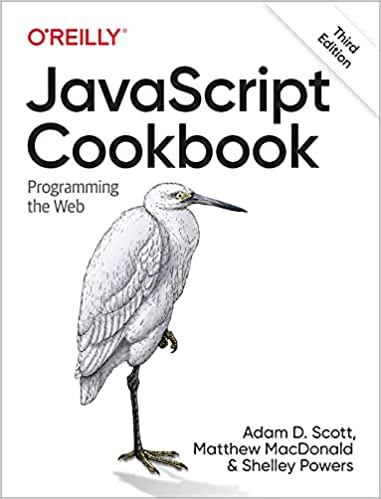
\includegraphics[width=6cm]{2021} 
\includegraphics[width=6cm]{2020a}\\
                
\includegraphics[width=6cm]{2020b} 
\includegraphics[width=6cm]{2018}\\
        {\tiny \sf Fonte: O autor }
    \end{center}
   \end{figure} 
    %%%%%%%%=================================
    \section{Vari\'{a}veis e constantes}
    %%%%%%%%=================================
    Uma variável é, de forma resumida, um nome simbólico para um valor armazenado no computador. Quando chamamos uma variável, estamos acessando o valor guardado por ela. \newline
    Na linguagem JavaScript, existem dois tipos de variáveis: as primitivas e as de objeto. 
    
    \subsection{Tipos Primitivos}
    
	Os tipos primitivos do JS incluem números, strings de textos e valores booleanos (true e false).
	Os tipos especiais null e undefined são valores primitivos, porém não são números, strings ou booleanos. Cada um é considerado membro de um tipo especial.  
	\subsubsection{Números}
	%TALVEZ Desconsiderar essa subsection
	\subsection{Tipos de Objeto}
	Na linguagem, qualquer valor que não seja um número, string, objeto ou null e undefined é um objeto. Um objeto é uma coleção de propriedades onde cda propriedade tem um nome e um valor.
	


    %%%%%%%%=================================
    \section{Tipos de Dados B\'{a}sicos}
    %%%%%%%%=================================

     %%%........................
            \subsection{String}
     %%%........................
            Um string \'{e} uma sequ\^{e}ncia de caracteres considerado como um item de dado simples. Para JavaScript, um string \'{e} um array de caracteres ou qualquer grupo de caracteres escritos entre doble aspas ou aspas simples. Por exemplo,
    \begin{lstlisting}
  <script type="text/javascript">
    var rows = prompt("How many rows for your multiplication table?");
    var cols = prompt("How many columns for your multiplication table?");
    if(rows == "" || rows == null)
   		 rows = 10;
    if(cols== "" || cols== null)
   		 cols = 10;
    createTable(rows, cols);
    function createTable(rows, cols)
    {
      var j=1;
      var output = "<table border='1' width='500' cellspacing='0'cellpadding='5'>";
      for(i=1;i<=rows;i++)
      {
    	output = output + "<tr>";
        while(j<=cols)
        {
  		  output = output + "<td>" + i*j + "</td>";
   		  j = j+1;
   		}
   		 output = output + "</tr>";
   		 j = 1;
    }
    output = output + "</table>";
    document.write(output);
    }
  </script>
\end{lstlisting}




     %%%%%%%%=================================
    \section{Tipos de Dados de Cole\c{c}\~{a}o}
    %%%%%%%%=================================


     %%%........................
            \subsection{Tipos Sequenciais}
     %%%........................


     %%%........................
            \subsection{Tipos Conjunto}
     %%%........................


     %%%........................
            \subsection{Tipos Mapeamento}
     %%%........................




    %%%%%%%%=================================
    \section{Estrutura de Controle e Fun\c{c}\~{o}es}
    %%%%%%%%=================================

     %%%........................
            \subsection{O comando IF}
     %%%........................


      %%%........................
            \subsection{La\c{c}o FOR}
     %%%........................

     %%%........................
            \subsection{La\c{c}o WHILE}
     %%%........................


    %%%%%%%%======================
    \section{M\'{o}dulos e pacotes}
    %%%%%%%%======================



       %%%........................
            \subsection{M\'{o}dulos}
     %%%........................



          %%%........................
            \subsection{Pacotes}
     %%%........................






    C\'{o}digo fonte para a linguagem JavaScript:
    \begin{lstlisting}
        <!DOCTYPE html>
        <html>
        <body>

        <h2>JavaScript Objects</h2>

        <p id="demo"></p>

        <script>
        var person = {
          firstName : "John",
          lastName  : "Doe",
          age     : 50,
          eyeColor  : "blue"
        };

        document.getElementById("demo").innerHTML =
        person.firstName + " is " + person.age + " years old.";
        </script>

        </body>
        </html>
    \end{lstlisting}





